\documentclass{beamer}
\usetheme{Montpellier}
\usecolortheme{beaver}
\title{Viscous Control of Shallow Elastic Fracture}
\author{Dominic Skinner}
\date{\today}
\begin{document}

\begin{frame}
\titlepage
\end{frame}

\begin{frame}{Introduction}
\begin{figure}
  \centerline{\includegraphics[scale=0.7]{./../Fig1.pdf}}
\end{figure}
\begin{itemize}
\item Set up: a semi-infinite elastic solid with a thin strip peeled off and 
      the resulting crack filled with an incompressible fluid
\item The motion is driven by a bending moment applied to the arm of the solid.
\end{itemize}
\end{frame}

\begin{frame}{Governing Equations}
Fluid Mechanics:
\begin{itemize}
\item Assume that the flow everywhere is in lubrication, i.e. Poiseulle
      flow in the crack. 
\item Look for travelling wave solutions with speed $c$. 
      Get the equation,
      $$ \frac{dp}{dx} = 12 \mu c /h^2 $$
\end{itemize}
Solid Mechanics:
\begin{itemize}
\item Assume the solid is a linear elastic solid. We can use Muskhelishiveli 
      methods to derive another equation,
      $$ \left[ \begin{array}{c} p \\ 0 \end{array} \right] 
      = \frac{E}{ 4\pi \ell (1-\nu^2) } \int_0^{\infty} \boldsymbol{K}
      (x - \tilde{x}) \left[ \begin{array}{c} g'(\tilde{x}) \\  h'(\tilde{x})
      \end{array} \right] d \tilde{x} . $$
\item $K_{ij}$ is the integral kernel specific to this geometry.
\end{itemize}
\end{frame}

\begin{frame}{Boundary conditions}
\begin{itemize}
\item The boundary conditions as $x \to \infty$ are governed by the bending 
      moment. We can use beam theory to approximate the elasticity equations 
      for $x$ large. This gives the boundary conditions
      $$ M(x) = \frac{E \ell^3}{12(1- \nu^2)} \frac{d^2 h}{dx^2} \to M_0 = 
      \mbox{ const.}$$
\item The boundary conditions as $x \to 0$ are govened by Linear Elastic 
      Fracture Mechanics, they are
      \[K_I = \lim_{x\to 0} \; \frac{E}{1-\nu^2}\sqrt{\frac{\pi}{8}} \sqrt{x}
      h'(x), \quad K_{II} = \lim_{x\to 0} \; \frac{E}{1-\nu^2}
      \sqrt{\frac{\pi}{8}} \sqrt{x} g'(x). \]
     
\end{itemize}
\end{frame}

\begin{frame}{Results}
\begin{figure}
  \centerline{\includegraphics[scale=0.8]{hprime-p-x-full.pdf}}
\end{figure}
\end{frame}

\begin{frame}{Speed vs. toughness}
\begin{itemize}
\item For a given bending moment, the speed should depend on the two
      toughness constants of the rock $K_I$, $K_{II}$ which correspond to
      mode $I$ and $II$ fracture respectively.
\item Actually have critical values of $K_I$ and $K_{II}$ for a given speed,
      only one of $K_I$, $K_{II}$ has to be equal to their critical values.
\item For example, if the critical values for $c=1$ were $(K_I,K_{II}) = 
      (1.3,1.5)$, then for both pairs of fracture constants: $(1.3, 20)$, 
      $(15,1.5)$, the speed would still be $1$.
\end{itemize}
\begin{center}
\includegraphics[scale=0.8]{./../NumFig3.pdf}
\end{center}
\end{frame}

\begin{frame}{Catagorising the toughness constants}
\begin{figure}
  \centerline{\includegraphics[scale=0.8]{catagory.pdf}}
\end{figure}
\begin{itemize}
\item There is a problem: the critical values only exist for 
      $K_{II} > 1.4$. So does that mean no travelling wave solutions
      for $K_{II} < 1.4$?
\item Actually something else happens, and a dry crack precedes the 
      wet tip, the ``two tip'' problem.
\end{itemize}
\end{frame}

\begin{frame}{Final Results}
\begin{figure}
  \centerline{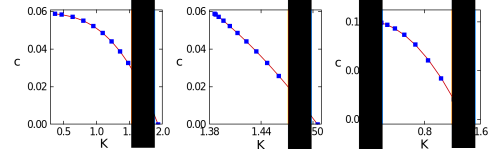
\includegraphics[scale=0.7]{overall-fit.pdf}}
\end{figure}
\end{frame}

\end{document}


